%___________________________________________
%*************************************************************
% Agent
%___________________________________________
%^^^^^^^^^^^^^^^^^^^^^^^^^^^^^^^^^^^^^^^^^^^^^^^^^^^

\section{Agent Framework}

%-----------------------------------------------------------------------
% Design
%-----------------------------------------------------------------------

\subsection{Design}
\label{subsec:agentdes}

\begin{figure}[t]
	\centering
	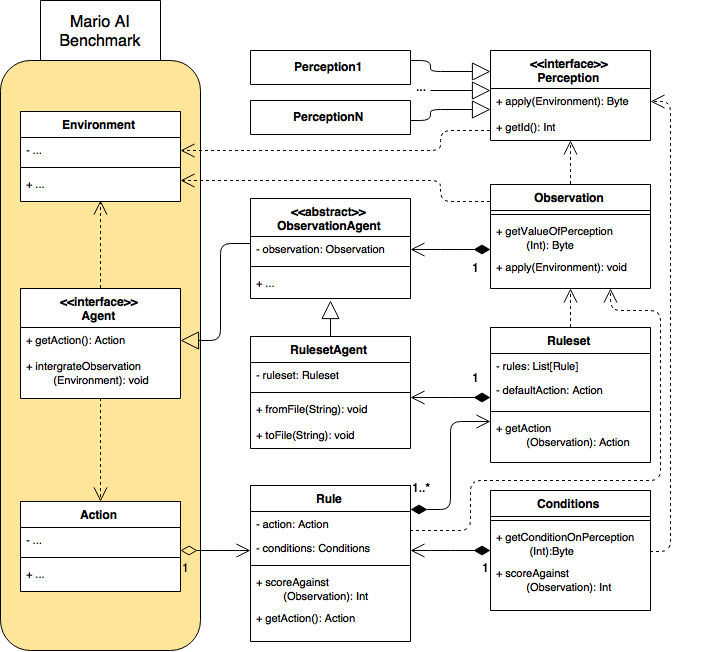
\includegraphics[scale=0.5]{AgentClassDiagram.png}
	\caption{UML class diagram of the agent framework.}
	\label{fig:aumlcd}
\end{figure}

The benchmark offers an \emph{Agent} interface, which when extended can be passed into the game playing portion of the software. Every game tick the current \emph{Environment} is passed to the agent, and then the agent is asked for an \emph{Action}, which is a set of explicit key press for Mario to perform.

The agent framework's basis will be extending this interface. Similar to REALM's agent, it will be a rule-based system. A UML class diagram of the system is given in Figure \ref{fig:aumlcd}.

\vspace{\baselineskip}

Each \emph{Agent} instance is initialised with a ruleset, consisting of a list of rules, each containing an \emph{Action}. On receiving the current game \emph{Environment} it is passed to a number of perception objects. Each one is responsible for a exactly one measurement (e.g. Enemy ahead, Mario moving to right etc.). These measurements are collected in to an observation object and stored in the agent.

When asked for an action, the \emph{Agent} passes this observation to its ruleset, which tests it against each rule. Rules contain conditions on what perception measurements should be, which determine its score for a given observation. The highest scoring rule (with a conflict strategy for ties) is then asked for its action, which is returned from the agent.

\vspace{\baselineskip}

Perceptions are hard coded; as such, all of an agents behaviour is determined by its ruleset. Thus, an implementation of the ruleset which allows persistence ensures that agents can be read and written to external files. Furthermore, rulesets are immutable and only information received during the current game tick is considered. Hence, agents have no state and are deterministic and thread safe (assuming the game engine is).

The capability of this framework is closely tied to the choice of perceptions. The more detail an agent is able to observe in its environment, the more potentially capable the agent can be. However, increasing the number of perceptions, and the detail they perceive at, increases the search space, making capable agents less likely to result from random mutation. Therefore, selection of perceptions must be careful considered, with a balance being struck between detail and brevity. 

The perceptions chosen were based upon those used in the REALM v1 agent \cite[p.~85]{realm}. The following is the final list of perceptions chosen:
\begin{description}
\item[MarioMode] Measures whether Mario is \textbf{small}, \textbf{big} or \textbf{fire} (capable of throwing fireballs).
\item[JumpAvailable] Detects if Mario has the ability to jump (i.e. on the ground or gripping a wall with the jump key off).
\item[OnGround] Measures whether Mario is in the air or not.
\item[EnemyLeft] Detects if an enemy is to the left of Mario.
\item[EnemyUpperRight] Detects if an enemy is to the upper right of Mario.
\item[EnemyLowerRight] Detects if an enemy is to the lower right or directly to the right of Mario.
\item[ObstacleAhead] Detects if there is a block or terrain directly to the right of Mario.
\item[PitAhead] Detects if there is a pit (falling into pits will end the level) to the right of Mario.
\item[PitBelow] Detects if there is a pit directly below Mario.
\item[MovingX] Measures the direction Mario is moving horizontally.
\item[MovingY] Measures the direction Mario is moving vertically.
\end{description}

The set of actions Mario can take is any combination of 6 key presses: \textbf{left}, \textbf{right}, \textbf{up}, \textbf{down}, \textbf{jump} and \textbf{speed} (which also shoots a fireball if possible). It was decided that this set would be restricted for use in the ruleset agent, only allowing cobinations of \textbf{left}, \textbf{right}, \textbf{jump} and \textbf{speed}. This was to reduce the size of the rules, which reduces the search space of any learning process. The \textbf{up} key performed no function and the \textbf{down} key made Mario crouch, which seemed too niche to be useful during the design process.


%-----------------------------------------------------------------------
% Lang + Tools
%-----------------------------------------------------------------------

\subsection{Language and Tools}

\subsubsection{Scala}
\label{subsec:langchoice}
The dependency on the Mario AI Benchmark restricts the language choice to those that can run on the JVM. Hence, Scala was chosen to be the primary language of the project. Its functional programming elements (pattern matching, list processing etc.) are very applicable to the ruleset and its semantic reasoner. Scala's focus on immutability aids in maintaining the thread safety requirement. Furthermore, ECJ's structure necessitates the use of type casting, which Scala handles elegantly. Several other Scala features were used throughout the project, such as lambdas, singletons, type aliases and case classes. 

\subsubsection{Maven}
With two major and several minor dependencies, their management is important to the project. Maven was chosen to maintain this, as well as package the main project and both the sub-projects. It was chosen for its ability to package both Java and Scala projects, keeping the tools consistent across the entire code base.


%-----------------------------------------------------------------------
% Impl
%-----------------------------------------------------------------------

\subsection{Implementation}

The design of the agent framework allows for agents to be fully determined by their ruleset. In order for an agent to be used in a evolutionary algorithm it must be represented by a simple data structure. Hence, implementation must allow for agent's rulesets to be unambiguously represented as, for example, a one dimensional collection. This section will describe the implementation steps taken to represent rulesets as a array of 8-bit integers, utilising Scala's built in types Vector and Byte.

\subsubsection{Perceptions}

The Perception interface was implemented as an abstract class, with an index integer field and an apply method. \emph{apply} takes the game Environment and returns a Byte (an 8-bit integer) instance, representing the measurement. Perception was extended into two further abstract classes: BoolPerception, which enforces apply's return be either 1 or 0, representing true and false respectively; and BytePerception, which has a limit field and enforces apply's return is between 0 and limit (inclusively). A full list of perceptions and what their byte values represent can be found in Table \ref{tab:AgKey} in Appendix \ref{app:percond}.

Concrete perceptions were implemented as objects (singletons) using the \emph{case} keyword, which allows for exhaustive pattern matching on the Perception class, as well as type safe extension by adding further case objects. Each one declares a unique index integer to the Perception superclass (starting at 0 and increasing by one for each). They implement the apply method to return their specific measurement. Figure \ref{fig:percumlcd} shows a class diagram of the this system.

\begin{figure}[t]
	\centering
	\includegraphics[scale=0.5]{PerceptionClassDiagram.png}
	\caption{UML class diagram of the perception system.}
	\label{fig:percumlcd}
\end{figure}

For illustration, consider these examples. The perception PitBelow extends BoolPerception, with a unique index of 8 and implements \emph{apply} to return 1 if there is a pit directly below Mario and 0 otherwise. MarioMode extends BytePerception, with a unique index of 0 and a limit of 2, with \emph{apply} returning 0 if Mario is \textbf{small}, 1 for \textbf{big} and 2 for \textbf{fire}.

This approach keeps all the information about perceptions contained in one file. The number of perceptions is easily extended by adding more case objects. Furthermore, it allows the Observation and Conditions classes to be implemented as fixed length byte vectors, with the vector's index matching the perception's unique index field. With use of Scala's implicit and extractor functionality, building the Observation and validating the Conditions vectors is type safe and concise:


\begin{minipage}{0.9\linewidth}
\centering
\begin{lstlisting}[language=scala]
val observationVector = 
    Vector.tabulate(Perception.NUMBER_OF_PERCEPTIONS) {
        n: Int => n match {
            // This retrieves the perception object with the index
            // that matches n. 
            case Perception(perception) => perception(environment)
        }
    }
\end{lstlisting}
\end{minipage}

\begin{minipage}{0.9\linewidth}
\centering
\begin{lstlisting}[language=scala]
def validateConditions(conditionsVector: Vector[Byte]): Boolean = {
    conditionsVector.zipWithIndex.forall {
        case (b: Byte, Perception(perception)) => perception match {
            case boolP : BoolPerception => 
                (b == boolP.TRUE) || (b == boolP.FALSE) 
                    || (b == DONT_CARE)
            case byteP : BytePerception => 
                ((0 <= b) && (b <= byteP.limit)) || (b == DONT_CARE)
        }
        case _ => false 
    }
}

\end{lstlisting}
\end{minipage}

Notice that no information about specific concrete perceptions is required, enforcing the open-closed design principle and allowing perceptions to be added without need to alter this code.

\subsubsection{Perceiving the Environment}

The \emph{Environment} interface contains several individual methods that report Mario's situation. Therefore implementing Perceptions that concerned Mario (e.g. MarioMode, MovingX etc.) was trivial.

Perceptions pertaining to enemies, obstacles or pits was more challenging. Environment provides two 19x19 arrays, one for enemies and one for terrain. Centred around Mario, each array element represents a `square' (16 pixels) of the level scene. The value of an element marks the presence of an enemy or terrain square. 

Enemy and obstacle perceptions pass the relevant array, a lambda test function, coordinates for a box segment of the array and a boolean to a helper function. This function uses Scala's for loop comprehensions to search through the box, applying the lambda to each element, returning the boolean parameter if the lambda returns true at least once. In this way it is easy to search for an enemy or obstacle in a box relative to Mario. Pits work in a similar way, but declare columns instead (see Listing \ref{lst:prcptpit} in Appendix \ref{app:percond}). If there is no terrain in the column below Mario's height, then it is considered a pit. Take EnemyLeft for example:

\begin{minipage}{0.9\linewidth}
\centering
\begin{lstlisting}[language=scala]
case object EnemyLeft extends BoolPerception(3) {
    // Minus = (Up,Left) | Plus = (Down,Right)
    val AREA_UL = (-2,-2); val AREA_BR = (1, -1);
  
    def apply(environment: Environment): Byte = {
        if(Perception.enemyInBoxRelativeToMario(environment, AREA_UL, AREA_BR)) 
            1 else 0  
    }
}
\end{lstlisting}
\end{minipage}

\begin{minipage}{0.9\linewidth}
\centering
\begin{lstlisting}[language=scala]
def enemyInBoxRelativeToMario(
          environment: Environment, 
          a: (Int, Int), b: (Int, Int)): Boolean = {
    val enemies = environment.getEnemiesObservationZ(2);
    val test = (grid: Array[Array[Byte]], tup: Tuple2[Int, Int]) =>{
         val x = grid(tup._1)(tup._2)
         x == 1
    }
    checkBox(enemies, test, getMarioPos(environment), a, b, true)
}
\end{lstlisting}
\end{minipage}

\begin{minipage}{0.9\linewidth}
\centering
\begin{lstlisting}[language=scala]
def checkBox(grid: Array[Array[Byte]], 
               test: (Array[Array[Byte]], (Int, Int))=>Boolean, 
               mario: (Int, Int), 
               a: (Int, Int), b: (Int, Int), 
               ret: Boolean): Boolean = {
    import Math.min
    import Math.max
    val relARow = min(grid.length-1, max(0, (a._1 + mario._1)))
    val relACol = min(grid(0).length-1, max(0, (a._2 + mario._2)))
    val relBRow = min(grid.length-1, max(0, (b._1 + mario._1)))
    val relBCol = min(grid(0).length-1, max(0, (b._2 + mario._2)))
    
    for {
      i <- min(relARow, relBRow) to max(relARow, relBRow)
      j <- min(relACol, relBCol) to max(relARow, relBCol)
      if (test(grid, (i, j)))
    }{
        return ret
    }
    !ret
}
\end{lstlisting}
\end{minipage}


\subsubsection{Observation, Conditions and Actions}

For clarity an Action class was created for use in the ruleset, with an adapter method to convert it into the boolean array expected in the Agent interface. As the Observation and Conditions classes were to be implemented as fixed length byte vectors, so was the Action class.

Action vectors have a fixed length of 4, where elements represent \textbf{left}, \textbf{right}, \textbf{jump} and \textbf{speed} respectively. Observation vectors have a fixed length equal to the number of perceptions and hold the byte returned by each Perception's apply function. Conditions have the same length and hold data in the same range as Observation, the condition on each perception therefore being that the corresponding element in the observation be equal. They have one additional possible value, {\footnotesize DONT\_CARE} (equal to byte -1), which represents that no condition be placed on that perception.

Instead of implementing these classes as wrappers for \emph{Vector[Byte]}, which can be inefficient and overly verbose, type aliases were used. This allowed each class to be referred to explicitly (rather than just by variable name), which provides readability and type safety, whilst still having direct access to the list processing methods included in the Vector class. They were declared on the agent framework's package object, making them accessible package wide. An object with static data and factory methods was included for each.

For example, this allowed Observation to be used as such:

\begin{minipage}{0.9\linewidth}
\centering
\begin{lstlisting}[language=scala]
abstract class ObservationAgent extends Agent {
    ...
    // Using factory method for a blank observation
    var observation: Observation = Observation.BLANK
    ...
    def integrateObservation{env: Environment}: Unit = {
        // Using the Observation factory method 
        // to build a new observation
        observation = Observation(env)
        
        if (printObservation) {
            // Using Vector method foreach directly
            observation.foreach { 
                b:Byte => print(" ~ " + b)
            }
        } 
        ...
    }
    ...
 }

\end{lstlisting}
\end{minipage}


\subsubsection{Rules and Rulesets}

Having both Conditions and Action implemented as byte vectors allows rules to be represented in the same way. Each rule is simple the concatenation of the Conditions and Action vectors. The rule vector are fixed length as both Conditions and Action are. Moreover, as rulesets contain just a list of rules, rulesets can be unambiguously represented by a single dimension byte vector. This allows rulesets not only to be persisted easily (as say a csv) but also gives the data representation needed for the evolutionary process.

In this case both Rule and Ruleset were implemented as wrapper classes for \emph{Vector[Byte]} and \emph{Seq[Rule]} respectively. Ruleset also holds a default Action, which is used if no rule matches the environment.

The semantic reasoner of the rule system is split across both classes. In Rule, the \emph{scoreAgainst} method is passed the observation and produces a score by looping through the conditions and adding 1 if the condition and observation match in value and 0 if the condition is {\footnotesize DONT\_CARE}. If a mismatched condition is found, the method immediately returns with -1. It is implemented tail recursively to provide maximum efficiency.

\begin{minipage}{0.9\linewidth}
\centering
\begin{lstlisting}[language=scala]
def scoreAgainst(observation: Observation): Int = {
    val conditions = ruleVector.slice(0, Conditions.LENGTH)
    @tailrec
    def scoreRecu(i: Int, sum: Int = 0): Int =  {
        if (i == Conditions.LENGTH) sum
        else conditions(i) match {
            case Conditions.DONT_CARE => scoreRecu(i+1, sum)
            case b if b == observation(i) => scoreRecu(i+1, sum+1)
            case _ => -1
        }
    }
    scoreRecu(0)
}
\end{lstlisting}
\end{minipage}

In Ruleset, the \emph{getBestAction} is passed the observation and returns an action boolean array. Using tail recursion it performs a fold operation on its rules, saving and returning the best scoring rule (preferring earlier rules when tied). If no rule gets a score of 0 or above then the default action is returned.

\begin{minipage}{0.9\linewidth}
\centering
\begin{lstlisting}[language=scala]
def getBestExAction(observation: Observation): Array[Boolean] = {
    
    @tailrec
    def getBestRuleRecu(rs: Seq[Rule], best: Option[Rule] = None, bestScore: Int = 0): Option[Rule] = 
        rs match {
          case Nil => best
          case (r +: ts) => {
              val newScore = r.scoreAgainst(observation)
              if (newRuleBetter(bestScore, newScore))
                  getBestRuleRecu(ts, Some(r), newScore)
              else
                  getBestRuleRecu(ts, best, bestScore)
        }
    }
\end{lstlisting}
\end{minipage}
    
\begin{minipage}{0.9\linewidth}
\centering
\begin{lstlisting}[language=scala]
    getBestRuleRecu(rules) match {
        case None => defaultAction.toBooleanArray
        case Some(r) => r.getAction.toBooleanArray
    }
}
\end{lstlisting}
\end{minipage}


\subsubsection{Persistence}

Agent's are persisted by persisting their ruleset. Rulesets are persisted in single line csv files. An IO helper object is passed an agent, extracts its ruleset and requests its vector representation, writing each byte separated by a comma. On reading an agent file, it constructs a byte vector. This byte vector is passed to the Ruleset's factory method, which groups the vector by rule length to form the rule sequence.

%-----------------------------------------------------------------------
% Testing
%-----------------------------------------------------------------------

\subsection{Testing}
\label{subsec:agenttest}

Due to the agent modules heavy reliance of the Environment interface the use of a mocking facility was required. The ScalaMock testing library was adding to the project to provide this.

Perceptions were unit tested individually, using white-box approach (due to the inclusion of mocking). Each test stubbed the Environment interface, instructing it to return a specific value (or array) for the relevant call, and testing that the perception echoed or processed it correctly. This allowed Perceptions to be tested independently of the game engine and provided test coverage. However, as there was very little documentation Environment interface, expected return values had to be investigated manually and edge cases could have easily been missed.

Rulesets (and Rules) were tested with a largely black-box end-to-end style. This was required due to the reliance of type aliases. Fixed rulesets were constructed to verify that the \emph{getAction} method returned the expected action based on a fixed observation. Mocking of individual rules was not used in case the Rule class was altered to be a type alias instead of a wrapper class.

These tests were added to Maven's build lifecycle, and hence run on every project build.

%-----------------------------------------------------------------------
% Handcrafted
%-----------------------------------------------------------------------

\subsection{Handcrafted Agents}
\label{subsec:hca}

For the purpose of evaluation and comparison three handcrafted rulesets were created for the agent framework. Full rulesets, as well as a key for condition values, can be found in Appendix \ref{app:har}.

\begin{description}
	\item[Forward Jumping] This ruleset commands the agent to jump whenever it can, regardless of its surroundings. It contains a single rule and a default action. It is a blind agent that does not take advantage of the framework, however it is surprising effective. An analogous agent was used for comparisons in the 2009 Mario AI Competition and was found to score higher than many entrants \cite[p.~7]{2010the}. The learning process will aim to discourage this behaviour as it is neither interesting or optimal.
	\item[Simple Reactive] This agent only jumps when it detects an enemy, obstacle or pit in its way. It contains 5 rules and defaults to moving right at speed. This agent makes better use of the framework, but still does not use all of its perceptions. Its behaviour is more interesting, however it tends to score similarly to the forward jumping agent. Despite low attainment, a learnt agent that behaves in a similar way will be evaluating more favourably as it is using more of the agent's perceptions.
	\item[Complex] This agent is the most interesting and highest scoring of the three. It has several different behaviours and builds off of the simple reactive agent. It contains 18 rules and makes use of all perceptions except MarioMode and EnemyLeft. Its behaviour was investigated at length and as such will form a good comparison to the final learnt agent. Effective evolved behaviours unconsidered in this agent's creation are a sign of the validity of the learning process. 
\end{description}
Creation of the handcrafted rulesets also informed additions and alterations to the agent's perceptions. For example, it was originally difficult to create an effective pit strategy and so PitAhead was changed from a BoolPerception to a BytePerception, returning 3 values representing \textbf{none}, \textbf{far} and \textbf{close}.

